\documentclass[letter]{article}
\usepackage[english]{babel}
\selectlanguage{english}
\usepackage[utf8]{inputenc}
\usepackage[T1]{fontenc}
\usepackage{color}
\usepackage{biblatex}
\usepackage[autostyle]{csquotes}
\addbibresource{sample.bib}
\usepackage[a4paper,top=3cm,bottom=2cm,left=3cm,right=3cm,marginparwidth=1.75cm]{geometry}
\usepackage{amsmath, amsthm, amsfonts}
\usepackage{graphicx}
\usepackage[colorinlistoftodos]{todonotes}
\usepackage[colorlinks=true, allcolors=blue]{hyperref}

\title{Solving the Problem of the Vertical Movement of a String Using Separation of Variables}
\author{Nicolás Díaz Durana}
\date{March 10, 2021}

\begin{document}
\maketitle
%%%%%%%%%%%%%%%%%%%%%%%%%%%%%%%%%%%%%%%%%%%%%%%%%%%%%%%%%%
\paragraph{}Using the method of separation of variables, we will solve the following problem:
    \begin{equation}
        \begin{split}
            u_{tt} &= c^2u_{tt},\\
            u(0,t) &= 0\\
            u(\ell,t) &= 0\\
            u(x,0) &= \phi(x)\\
            u_t(x,0) &= \psi(x)
        \end{split}
    \end{equation}
    \paragraph{}where $0<x<\ell$, $t>0$ and $\phi(0)=\phi(\ell)=\psi(0)=\psi(\ell)=0$.\\
    \paragraph{}\textbf{Preliminary Analysis}
    \paragraph{}This problem describes the vertical movement of a string with length $\ell$ from the $x$ axis at a position $x$  and a time $t$. The ends of the string are held fix, where the left end of the string is $x=0$ and the right end is $x=\ell$.
    \begin{center}     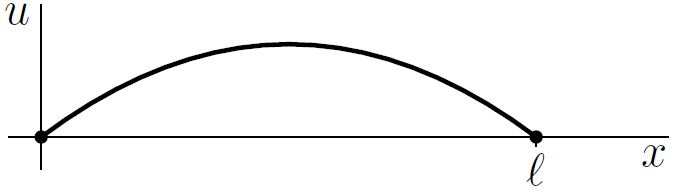
\includegraphics[width=.35\textwidth]{wave_func.JPG}
    \end{center}
    \paragraph{}If the string undergoes small amplitude vibrations, then we can assume that $u(x,t)$ behaves under the wave equation:
    \begin{equation}
        \begin{split}
            \frac{\partial^2u}{\partial t^2}(x,t) &= c^2\frac{\partial^2}{\partial x^2}(x,t)
        \end{split}
    \end{equation}
    with $0<x<\ell$ and $t>0$.
    \paragraph{} The boundary conditions are given by
    \begin{equation}
        \begin{split}
            u(0,t) &= 0\\
            u(\ell,t) &= 0\\
        \end{split}
    \end{equation}
    meaning that the string is held at a height $0$ in both its ends.
    \paragraph{} The initial conditions are given by
        \begin{equation}
        \begin{split}
            u(x,0) &= \phi(x)\\
            u_t(x,0) &= \psi(x)
        \end{split}
    \end{equation}
    which refer to the position and the speed of the string at the time $0$.
    \paragraph{}We want to find $u(t,x)$ for all $x$ and $t$. To this end, we will use the method of separation of variables, following three steps:
    \begin{enumerate}
        \item Find all solutions of (2) that satisfy the form $u(x,t)=X(x)T(t)$, for some $X(x)$ that only depends on position and some $T(t)$ that only depends on time.
        \item Evaluate the boundary conditions given in (3)
        \item Evaluate the initial conditions given in (4)
    \end{enumerate}
    %%%%%%%%%%%%%%%%%%%%%%%%%%% Punto 1
    \paragraph{}\textbf{Solving the equation}
    \paragraph{}We will begin by rewriting the function $u(x,t)=X(x)T(t)$ as:
    \begin{equation}
        \begin{split}
            X(x)T''(t) & =c^2X''(x)T(t) \\
            \frac{X''(x)}{X(x)} &= \frac{1}{c^2}\frac{T''(t)}{T(t)}\\
        \end{split}
    \end{equation}
    \paragraph{}We notice that the right side of (5) is independent of $X$, whereas the left side is independent of $t$. Which means that both sides must be constant. We will call this constant $\omega$:
    \begin{equation}
        \begin{split}
            \frac{X''(x)}{X(x)} &= \frac{1}{c^2}\frac{T''(t)}{T(t)} =0\\
            & \Rightarrow X''(x)-\omega X(x) = 0\\
            & \Rightarrow T''(t)-c^2\omega T(t)=0
        \end{split}
    \end{equation}
    \paragraph{}Now we have two ordinary differential equations, which we will proceed to solve:
    \begin{enumerate}
    %%%%%%%%%%%%%%%%%%%%%%
        \item \textbf{$X''(x)-\omega X(x) = 0$}
        \\ \\Assuming $X(x)=e^{rx}$ for some unknown $r$
        \begin{equation}
            \begin{split}
                \frac{d^2}{dx^2}e^{rx}-\omega e^{rx} &= 0\\
                (r^2-\omega)e^{rx} &= 0\\
                r^2 - \omega &= 0\\
                r &= \pm \sqrt{\omega}\\
                \text{Therefore, the general solution for X(x) is:}\\
                X(x) &= p_1e^{\sqrt{\omega}x}+p_2e^{-\sqrt{\omega}x}
            \end{split}
        \end{equation}
        
    %%%%%%%%%%%%%%%%%%%%%%    
        \item \textbf{$T''(t)-c^2\omega T(t)=0$}
        \\ \\Assuming $T(t)=e^{st}$ for some unknown $s$:
        \begin{equation}
            \begin{split}
                \frac{d^2}{dx^2}e^{st}-c^2\omega e^{st} &= 0\\
                (s^2-c^2\omega)e^{st} &= 0\\
                s^2 - c^2\omega &= 0\\
                s &= \pm c\sqrt{\omega}\\
                \text{Therefore, the general solution for T(t) is:}\\
                T(t) &= p_3e^{c\sqrt{\omega}t}+p_4e^{-c\sqrt{\omega}t}
            \end{split}
        \end{equation}
    \end{enumerate}
    \paragraph{} In the previous solutions, $p_1,p_2,p_3,p_4$ are arbitrary constants and $\omega\neq0$.
    \paragraph{} If $\omega=0$, we get the trivial solutions where $X''(x)=0$ and $T''(t)=0$, plus the general solution:
    \begin{equation}
        \begin{split}
            X(x) &= p_1+p_2x\\
            T(t) &= p_3+p_4t
        \end{split}
    \end{equation}
    \paragraph{}Putting both results back together, we get the set of solutions for equation (2):
    \begin{equation}
        \begin{split}
            u(x,t) 
            &= (p_1e^{\sqrt{\omega}x}+p_2e^{-\sqrt{\omega}x})(p_3e^{c\sqrt{\omega}t}+p_4e^{-c\sqrt{\omega}t})\text{, }\omega \neq 0\\
            u(x,t) 
            &= (p_1+p_2x)(p_3+p_4t)
        \end{split}
    \end{equation}
    
    %%%%%%%%%%%%%%%%%%%%%%%%%%%
    
    \paragraph{}\textbf{Evaluating the Boundary Conditions}
    \paragraph{}Recall the boundary conditions defined in (3):
        \begin{equation*}
        \begin{split}
            u(0,t) &= 0\\
            u(\ell,t) &= 0\\
        \end{split}
    \end{equation*}
    \paragraph{}Since $X_i(x)T_i(t)$, $i=1,2,3,...,n$ all solve the equation (2), it follows that $\sum_i a_i X_i(x)T_i(t)$ also will lead to solutions for any constant $a$. Therefore,
    \begin{equation}
        \begin{split}
            \sum_i a_i X_i(0)T_i(t) &= 0 \qquad \text{for all } t>0
        \end{split}
    \end{equation}
    satisfies the boundary condition $u(0,t)=0$.
    \paragraph{}Likewise, 
    \begin{equation}
        \begin{split}
            \sum_i a_i X_i(\ell)T_i(t) &= 0 \qquad \text{for all } t>0
        \end{split}
    \end{equation}
    satisfies the boundary condition $u(\ell,t)=0$.
    \paragraph{}We are now interested in knowing which of the solutions that we found in (10) satisfy $X(0)=X(\ell)=0$
    \paragraph{}Let's consider $\omega=0$, so that $X(x)=p_1+p_2x$. The condition $X(0)=X(\ell)=0$ is only satisfied if and only if $p_1=p_2=0$. But this trivial solution does not interest us, so we are going to discard $\omega=0$.
    \paragraph{} Now, consider $\omega \neq 0$, so that $p_1e^{\sqrt{\omega}x}+p_2e^{-\sqrt{\omega}x}$. Here we see that the condition $X(0)=0$ can only be satisfied if $p_1+p_2=0$, which means that $p_2=-p_1$.
    \paragraph{}Similarly, the condition $X(\ell)=0$ is satisfied if and only if
    \begin{equation}
        \begin{split}
            0=p_1e^{\sqrt{\omega}\ell}+p_2 e^{-\sqrt{\omega}\ell} 
            &= p_1(e^{\sqrt{\omega}\ell}-e^{-\sqrt{\omega}\ell})
        \end{split}
    \end{equation}
    \paragraph{}Once again, we want to discard any trivial solutions: for example, when $p_1=0$. Therefore, we will only settle for values of $\omega$ that satisfy
    \begin{equation}
        \begin{split}
            e^{\sqrt{\omega}\ell}-e^{-\sqrt{\omega}\ell} 
            = 0 &\Longleftrightarrow e^{\sqrt{\omega}\ell}=e^{-\sqrt{\omega}\ell}\\
            &\Longleftrightarrow e^{2\sqrt{\omega}\ell}=1
        \end{split}
    \end{equation}
    \paragraph{}For this reason, we discard $\omega=0$. So $e^{2\sqrt{\omega}\ell}=1$ if there exists and integer $k$ such that
    \begin{equation}
        \begin{split}
            2\sqrt{\omega}l = 2p\pi i 
            &\Longleftrightarrow \sqrt\omega =k\frac{\pi}{\ell}i\\
            &\Longleftrightarrow \omega = -k^2\frac{\pi^2}{\ell^2}
        \end{split}
    \end{equation}
    \paragraph{}Taking $\sqrt{\omega}=k\frac{\pi}{\ell}i$ and $p_2=-p_1$, we get
    \begin{equation*}
        \begin{split}
            X(x)T(t) 
            &= p_1\bigg(e^{i\frac{k\pi}{\ell}x}-e^{-i\frac{k\pi}{\ell}x}\bigg)\bigg(p_3e^{i\frac{ck\pi}{\ell}t}-p_4e^{-i\frac{ck\pi}{\ell}t}\bigg)\\
            &= 2ip_1\text{sin}\bigg(\frac{k\pi}{\ell}x\bigg)\bigg[\big(p_3+p_4\big)\text{cos}\bigg(\frac{ck\pi}{\ell}t\bigg)+i\big(p_3-p_4\big)\text{sin}\frac{ck\pi}{\ell}t\bigg]\\
            &= \text{sin}\bigg(\frac{k\pi}{\ell}x\bigg)\bigg[\alpha_k\text{cos}\bigg(\frac{ck\pi}{\ell}t\bigg)+\beta_k\text{sin}\bigg(\frac{ck\pi}{\ell}t\bigg)\bigg]
        \end{split}
    \end{equation*}
    where $\alpha_k=2ip_1(p_3+p_4)$ and $\beta_k=-p_1(p_3-p_4)$, with $p_1,p_3,p_4,\alpha_k,\beta_k\in\mathbb{C}$\\
    
    %%%%%%%%%%%%%%%%%%%%%%%%%%%
    
    \paragraph{}\textbf{Imposing the Initial Conditions}
    \paragraph{} Recall the initial conditions defined in (4):
        \begin{equation*}
        \begin{split}
            u(x,0) &= \phi(x)\\
            u_t(x,0) &= \psi(x)
        \end{split}
    \end{equation*}
    \paragraph{}We have seen that the wave equation (2) and the given boundary conditions (3) successfully adapt to
    \begin{equation}
        \begin{split}
            u(x,t) &= 
            \sum_{k=1}^\infty\text{sin}\bigg(\frac{k\pi}{\ell}x\bigg)\bigg[\alpha_k\text{cos}\bigg(\frac{ck\pi}{\ell}t\bigg)+\beta_k\text{sin}\bigg(\frac{ck\pi}{\ell}t\bigg)\bigg]
        \end{split}
    \end{equation}
    where $\alpha_k,\beta_k$ are arbitrary constants. 
    \paragraph{}Now, we need to find values for $\alpha_k,\beta_k$ that satisfy the given initial conditions, such that
    \begin{equation}
        \begin{split}
            \phi(x) &= u(x,0) = \sum_{k=1}^\infty\alpha_k\text{ sin}\bigg(\frac{k\pi}{\ell}x\bigg)
        \end{split}
    \end{equation}
    \begin{equation}
        \begin{split}
            \psi(x) &= u_t(x,0) = \sum_{k=1}^\infty\beta_k\frac{ck\pi}{\ell}\text{ sin}\bigg(\frac{k\pi}{\ell}x\bigg)
        \end{split}
    \end{equation}
    \paragraph{} To achieve this, first note that any function defined on the interval $0<x<\ell$ fits the following unique representation as a linear combination of $\text{sin}\frac{k\pi x}{\ell}$:
    \begin{equation}
        \begin{split}
            \xi(x) &= \sum_{k=1}^\infty b_k\text{ sin}\frac{k\pi x}{\ell}
        \end{split}
    \end{equation}
    \paragraph{}Additionally, we know the formula for the coefficients
    \begin{equation*}
        \begin{split}
            b_k &= \frac{2}{\ell}\int_{0}^{\ell}\xi(x)\text{ sin}\frac{k\pi x}{\ell}dx
        \end{split}
    \end{equation*}
    \paragraph{}So, we can combine (17) and (19) by considering $\phi(x)=\xi(x)$ and $b_k=\alpha_k$:
    \begin{equation}
        \begin{split}
            \alpha_k &= \frac{2}{\ell}\int_{0}^{\ell}\phi(x)\text{ sin}\frac{k\pi x}{\ell}dx
        \end{split}
    \end{equation}
    \paragraph{}Similarly, we can make (18) and (19) match by considering $\psi(x)=\xi(x)$ and $b_k=\beta_k\frac{ck\pi}{\ell}$:
    \begin{equation}
        \begin{split}
            \beta_k &= \frac{2}{ck\pi}\int_{0}^{\ell}\psi(x)\text{ sin}\frac{k\pi x}{\ell}dx
        \end{split}
    \end{equation}
    \paragraph{}With these values of $\alpha_k$ (20) and $\beta_k$ (21) associated to the sum in the equation (16) 
    \begin{equation*}
        \begin{split}
            u(x,t) &= 
            \sum_{k=1}^\infty\text{sin}\bigg(\frac{k\pi}{\ell}x\bigg)\bigg[\alpha_k\text{cos}\bigg(\frac{ck\pi}{\ell}t\bigg)+\beta_k\text{sin}\bigg(\frac{ck\pi}{\ell}t\bigg)\bigg]
        \end{split}
    \end{equation*}
    \paragraph{}we have reached a final solution.\\
\end{document}